% !TeX spellcheck = it_IT
\documentclass[a4paper]{article}
\usepackage{amsmath}
\usepackage{pgfplots}
\usepackage[italian]{babel}

\title{FONDAMENTI DI MATEMATICA}
\author{Enrico Martini}
\date{v1.0 | 2015 - 2019}


\begin{document}
	
	\maketitle
	\thispagestyle{empty}
	\newpage
	\tableofcontents
	\thispagestyle{empty}
	\newpage
	
	\section{Geometria analitica}
	\subsection{Punto}
	Rappresentazione:
	\begin{align*}
		P(x_P;y_P)
	\end{align*}
	Distanza tra due punti:
	\begin{align*}
		d = \sqrt{(x_B -x _A)^2+(y_B - y_A)^2}
	\end{align*}
	Punto medio:
	\begin{align*}
		M \left( \frac{x_A + x_B}{2} ; \frac{y_A + y_B}{2} \right)
	\end{align*}
	Baricentro:
	\begin{align*}
		G \left( \frac{x_A + x_B + x_C}{3} ; \frac{y_A + y_B + y_C}{3} \right) 
	\end{align*}
	Area di un triangolo:
	\begin{align*}
		A = \frac{1}{2} \cdot \left| \begin{array}{cc}
		x_C-x_A & y_C-y_A \\ 
		x_B-x_A & y_B-y_A
		\end{array} \right|
	\end{align*}
	
	\subsection{Retta}
	Rappresentazione:
	\begin{align*}
		y &= mx + q		&\vee&&		ax + by + c & = 0
	\end{align*}
	Retta passante per due punti:
	\begin{align*}
		\frac{y-y_A}{y_B-y_A} = \frac{x-x_A}{x_B-x_A}
	\end{align*}
	Fascio di rette passante per un punto:
	\begin{align*}
		y-y_0 = m(x-x_0)
	\end{align*}
	Distanza punto-retta:
	\begin{align*}
		d = \frac{|ax_0+by_0+c|}{\sqrt{a^2+b^2}}
	\end{align*}
		
	\subsection{Circonferenza}
	Rappresentazione:
	\begin{align*}
		x^2+y^2+ax+by+c&=0	& (x-\alpha)^2 + (y-\beta)^2 &= r^2
	\end{align*}
	Coordinate del centro:
	\begin{align*}
		C \left( -\frac{a}{2} ; -\frac{b}{2} \right)
	\end{align*}
	Raggio:
	\begin{align*}
		r = \frac{1}{2}\sqrt{a^2+b^2-4c}
	\end{align*}
	
	\subsection{Parabola}
	Rappresentazione:
	\begin{align*}
		y &= ax^2 + bx + c		&		x &= ay^2 + by + c
	\end{align*}
	Vertice:
	\begin{align*}
		V& \left(-\frac{b}{2a};-\frac{\varDelta}{4a}\right)		&		V & \left( -\frac{\varDelta}{4a} ; -\frac{b}{2a} \right) 
	\end{align*}
	
	\subsection{Ellisse}
	Rappresentazione:
	\begin{align*}
		\frac{x^2}{a^2} + \frac{y^2}{b^2} = 1
	\end{align*}
	Con $a>b$:
	\begin{align*}
		F&(\pm c ; 0)		&		c = \sqrt{a^2-b^2}
	\end{align*}
	Con $a < b$:
	\begin{align*}
		F&(0 ; \pm c)		&		c = \sqrt{b^2-a^2}
	\end{align*}
	
	\subsection{Iperbole}
	Rappresentazione:
	\begin{align*}
	\frac{x^2}{a^2} - \frac{y^2}{b^2} = 1
	\end{align*}
	Se rivolta all'asse $x$:
	\begin{align*}
		F&(\pm c ; 0)		&		c^2 &= a^2 + b^2		&		y &= \pm \frac{b}{a}x
	\end{align*}
	Se equilatera:
	\begin{align*}
		x^2 - y^2 &= a^2		&		y &= \pm x
	\end{align*}
	
	\subsubsection{Funzione omografica}
	Rappresentazione:
	\begin{align*}
	y &= \frac{ax + b}{cx + d}		&		C&\left( -\frac{d}{c} ; \frac{a}{c} \right)
	\end{align*}
	
	\subsection{Coniche generali}
	\begin{align*}
		ax^2+bxy+cy^2+dx+ey+f=0
	\end{align*}
	
	
	
	\newpage	
	\section{Trasformazioni geometriche}
	\subsubsection*{Simmetria}
	 Simmetria rispetto ad un punto $P(\alpha , \beta)$ :
	 \begin{align*}
	 	\begin{cases}
	 	x' = 2 \alpha - x \\
	 	y' = 2 \beta -y 
	 	\end{cases}
	 \end{align*}
	 Simmetria rispetto all'asse $y$:
	 \begin{align*}
	 	\begin{cases}
	 	x' = -x\\
	 	y' = y
	 	\end{cases}
	 \end{align*}
	Simmetria rispetto all'asse $x$:
	\begin{align*}
		\begin{cases}
			x' = x\\
			y' = -y
		\end{cases}
	\end{align*}
	
	\subsubsection*{Traslazione}
	Traslazione rispetto ad un vettore $\vec{v} (a;b)$:
	\begin{align*}
		\begin{cases}
			x'=x+a\\
			y'=y+b
		\end{cases}
	\end{align*}
	
	\subsubsection*{Rotazione}
	Rotazione rispetto ad un angolo $\alpha$:
	\begin{align*}
		\begin{cases}
			x=x' \cdot \cos (\alpha) + y' \cdot \sin(\alpha)\\
			y= -x' \cdot \sin (\alpha) + y' \cdot \cos(\alpha)
		\end{cases}&
		\begin{cases}
			x'= x \cdot \cos (\alpha) - y \cdot \sin(\alpha)\\
			y'= x \cdot \sin (\alpha) + y \cdot \cos(\alpha)
		\end{cases}
	\end{align*}
	\subsubsection*{Omotetia}
	Omotetia di centro $O(0;0)$ e rapporto $h$:
		\begin{align*}
	\begin{cases}
	x' = hx - x_c\\
	y' = hx - y_c
	\end{cases}
	\end{align*}
	\subsubsection*{Affinità}
	\begin{align*}
		&\begin{cases}
			x'=ax+by+h\\
			y'=cx+dy+k
		\end{cases}&
		con &\varDelta = \left| \begin{matrix}
		a & b \\ 
		c & d
		\end{matrix}
		\right|\neq 0
	\end{align*}
	
	\newpage
	\section{Solidi}
	\subsubsection*{Cilindro}
	\begin{align*}
		S_L & = 2p \cdot h & S_{TOT} & = S_L + 2S_B  \\
		S_B & = \pi r^2    & V       & = S_b \cdot h
	\end{align*}
	\\
	\subsubsection*{Cono}
	\begin{align*}
		S_L & = \pi r a & S_{TOT} & = S_L + 2S_B            \\
		S_B & = \pi r^2 & V       & = \frac{1}{3} \pi r^2 h
	\end{align*}
	\\
	\subsubsection*{Sfera}
	\begin{align*}
		S &= 4\pi r^2 & V &= \frac{4}{3} \pi r^3
	\end{align*}
	\\
	\subsubsection*{Prisma}
	\begin{align*}
		S_L &= 2p \cdot h	&	S_{TOT} &= S_L +2S_B
		&			V &= S_b \cdot h
	\end{align*}
	\\
	\subsubsection*{Piramide}
	\begin{align*}
		S_L &= pa	&	S_{TOT} &= S_L + S_B\\
		S_B &= l^2	&	V &= \frac{1}{3} S_B \cdot h
	\end{align*}
	
	\newpage
	\section{Geometria analitica dello spazio}

	\subsubsection*{Equazione del piano}
	\begin{align*}
		\alpha : ax +by +cz+ d &= 0			&			d &= -a^2-b^2-c^2
	\end{align*}

	\subsubsection*{Punto medio}
	\begin{align*}
		M \left( \frac{x_A + x_B}{2} ; \frac{y_A + y_B}{2} ; \frac{z_A + z_B}{2} \right)
	\end{align*}

	\subsubsection*{Equazione di una retta}
	\begin{align*}
		\begin{cases}
		ax+by+cz+d=0\\
		ex+fy+gz+h=0
		\end{cases}
	\end{align*}

	\subsubsection*{Retta passante per due punti}
	\begin{align*}
		\frac{x - x_A}{x_B - x_A} = \frac{y - y_A}{y_B - y_A} = \frac{z - z_A}{z_B - z_A} = \lambda
	\end{align*}

	\subsubsection*{Distanza tra piano e punto}
	\begin{align*}
		d(A ; \alpha) = \frac{|ax_A + by_A + cz_A + d|}{\sqrt{a^2+b^2+c^2}}
	\end{align*}
	
	\subsubsection*{Piano parallelo ad un altro piano passante per un punto}
	
	\begin{align*}
	\alpha = \left|
		\begin{array}{ccc}
			a & b & c \\ 
			a' & b' & c' \\ 
			a'' & b'' & c''
		\end{array}
		\right| = 0 
	\end{align*}
		
	\subsubsection*{Retta perpendicolare ad un piano passante per un punto}
	
	\begin{align*}
		\frac{x-x_0}{a} = \frac{y-y_0}{b} = \frac{z-z_0}{c}
	\end{align*}
	
	\subsubsection*{Piano passante per un punto perpendicolare ad una retta}
	
	\begin{align*}
		\alpha = l(x-x_0)+m(y-y_0)+n(z-z_0)=0
	\end{align*}
	
	\subsubsection*{Parallelismo tra piani}
	\begin{align*}
		\frac{a}{a'} = \frac{b}{b'} = \frac{c}{c'} \ne \frac{d}{d'}
	\end{align*}
	
	\subsubsection*{Perpendicolarità tra piani}
	\begin{align*}
		aa'+bb'+cc'=0
	\end{align*}
	
	\newpage
	\section{Probabilità}
	\begin{align*}
		p(E) & = \frac{casi_{POSSIBILI}}{casi_{TOTALI}} & 0 & \le p(E) \le 1
	\end{align*}
	
	\subsubsection*{Probabilità della somma logica di eventi}
	\begin{align*}
		p(E_1 \cup E_2) = p(E_1) + p(E_2) - p(E_1 \cap E_2)
	\end{align*}
	
	\subsubsection*{Probabilità condizionata}
	\begin{align*}
		p(E_1 | E_2) = \frac{p(E_1 \cap E_2)}{p(E_2)}
	\end{align*}
	
	\subsubsection*{Probabilità del prodotto logico di eventi}
	\begin{align*}
		\begin{cases}
		p(E_1 \cap E_2) = p(E_1) \cdot p(E_1 | E_2)	& dipendenti\\
		p(E_1 \cap E_2) = p(E_1) \cdot p(E_2)		& indipendenti
		\end{cases}
	\end{align*}
	
	\subsubsection*{Problema delle prove ripetute}
	\begin{itemize}
		\item n : numero di estrazioni
		\item k : numero delle volte in cui deve uscire
		\item p : probabilità che si verifichi
		\item q : probabilità che non si verifichi
	\end{itemize}

	\begin{align*}
		P_{k,n} = {{n}\choose{k}} p^kq^{n-k}
	\end{align*}
	
	\subsubsection*{Teorema di Bayes}
	\begin{align*}
		p(E_i|E)= \frac{p(E_i) \cdot p(E | E_i)}{p(E)}
	\end{align*}
	
	\newpage
	\section{Calcolo combinatorio}
	\subsubsection*{Disposizione semplice}
	Tutti i gruppi con $k$ elementi su $h$ elementi diversi per contenuto e ordine non ripetuti.
	\begin{align*}
		D_{n,k} = n(n-1)(n-2)...(n-k+1)
	\end{align*}

	\subsubsection*{Disposizione con ripetizione}
	\begin{align*}
		D'_{n,k} = n^k
	\end{align*}

	\subsubsection*{Permutazione semplice}
	Tutti i gruppi con $n$ elementi con ordine diverso.
	\begin{align*}
		P_n = n! 
	\end{align*}
	
	\subsubsection*{Permutazione con ripetizione}
	\begin{align*}
		P_n^{(n;k)}=\frac{n!}{n!k!}
	\end{align*}
	
	\subsubsection*{Combinazione semplice}
	Scegliere $k$ elementi su $n$, senza ripetizione e senza cambiare l'ordine.
	\begin{align*}
		C_{n,k} = {{n}\choose{k}} = \frac{D_{n,k}}{P_k} = \frac{n(n-1)(n-2)...(n-k+1)}{k!} 
	\end{align*}
	
	\subsubsection*{Combinazione con ripetizione}
	\begin{align*}
		C'_{n,k} = C_{n+k-1 , k} = {{n+k-1}\choose{k}}
	\end{align*}
	
	\newpage
	\section{Goniometria}
		
	Formula fondamentale:
	\begin{align*}
	\sin ^2 (\alpha) + \cos^2 (\alpha) = 1
	\end{align*}
	Formule derivate:
	\begin{align*}
	\tan (\alpha) & = \frac{\sin (\alpha)}{\cos (\alpha)} & \cot (\alpha) & = \frac{\cos (\alpha)}{\sin (\alpha)} \\
	\sec (\alpha) & = \frac{1}{\sin (\alpha)}             & \csc (\alpha) & = \frac{1}{\cos (\alpha)}
	\end{align*}
	Somma e differenza:
	\begin{align*}
	\sin (\alpha + \beta) & = \sin (\alpha) \cdot \cos (\beta) + \cos (\alpha) \cdot \sin (\beta)\\
	\cos (\alpha + \beta) & = \cos (\alpha) \cdot \cos (\beta) - \sin (\alpha) \cdot \sin (\beta)\\
	\sin (\alpha - \beta) & = \sin (\alpha) \cdot \cos (\beta) - \cos (\alpha) \cdot \sin (\beta)\\
	\cos (\alpha - \beta) & = \cos (\alpha) \cdot \cos (\beta) + \sin (\alpha) \cdot \sin (\beta)
	\end{align*}
	Duplicazione:
	\begin{align*}
	\sin (2 \alpha) & = 2 \sin (\alpha) \cdot \cos (\alpha)	&	\cos (2 \alpha) & = \cos^2 (\alpha) - \sin^2 (\alpha)
	\end{align*}
	Bisezione:
	\begin{align*}
	\cos \left(\frac{\alpha}{2}\right) &= \pm \sqrt{\frac{1 + \cos (\alpha)}{2}} & \sin \left(\frac{\alpha}{2}\right) &= \pm \sqrt{\frac{1 - \cos (\alpha)}{2}}\\
	\tan \left(\frac{\alpha}{2}\right) &= \pm \sqrt{\frac{1-\cos (\alpha)}{1+\cos (\alpha)}} = &\frac{\sin (\alpha)}{1+\cos (\alpha)} &= \frac{1-\cos (\alpha)}{\sin (\alpha)}
	\end{align*}
	Formule parametriche:
	\begin{align*}
	\sin (\alpha) &= \frac{2t}{1+t^2} & \cos (\alpha) = \frac{1 - t^2}{1 + t^2} & & t= \tan \left(\frac{\alpha}{2}\right)
	\end{align*}
	
	\begin{center}
		\begin{tikzpicture}
		\begin{axis}[
		axis lines = left,
		xlabel = $x$,
		ylabel = {$f(x)$},
		]
		
		\addplot [
		domain= 0:6.28,
		samples=100, 
		color=red,
		]
		{sin(deg(x))};
		\addlegendentry{$\sin (x)$}
		
		\addplot [
		domain=0:6.28, 
		samples=100, 
		color=blue,
		]
		{cos(deg(x))};
		\addlegendentry{$\cos(x)$}
		
		\end{axis}
		\end{tikzpicture}
	\end{center}
	
	\begin{center}
		\begin{figure}
			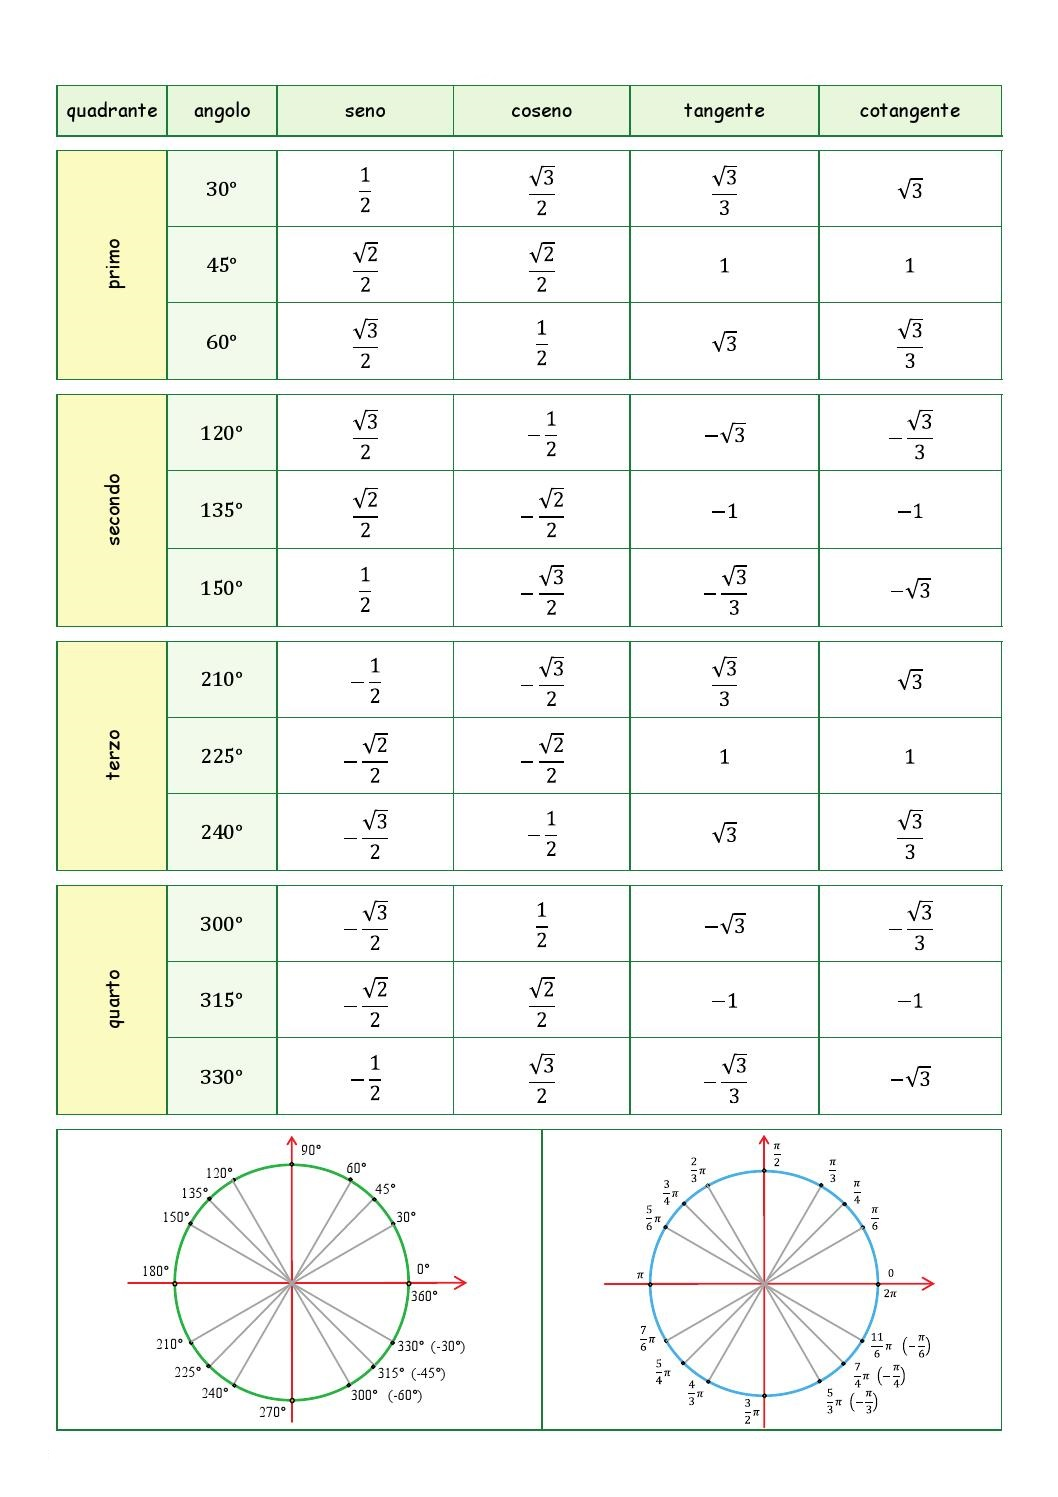
\includegraphics[width=\linewidth]{sincos.jpg}
			\caption{Tabella degli angoli associati}
		\end{figure}
	\end{center}
	
	
	\newpage
	\section{Trigonometria}

	\begin{figure}[htbp]
		\begin{center}
			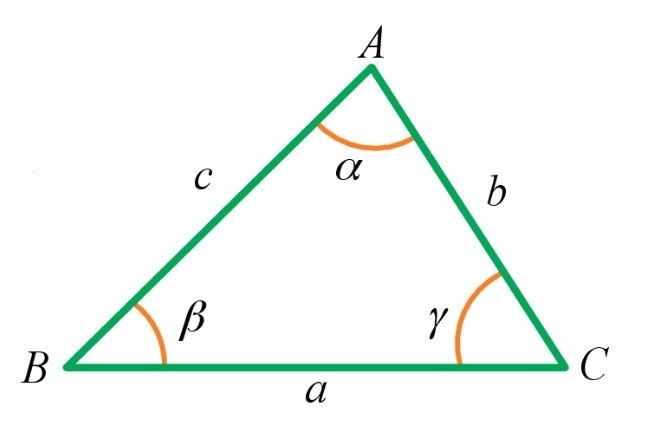
\includegraphics[width=\linewidth]{trigonometria.jpg}
		\end{center}
	\end{figure}



	\subsubsection*{Teorema dei seni}
	\begin{align*}
	\frac{a}{\sin \alpha} = \frac{b}{\sin \beta} = \frac{c}{\sin \gamma}
	\end{align*}
	
	\subsubsection*{Teorema del coseno}
	\begin{align*}
		a^2 = b^2 + c^2 -2bc\cos \alpha
	\end{align*}
	
	\newpage
	\section{Esponenziali}
	\begin{align*}
		a^x &= b		&		a>&0
	\end{align*}
		
			\begin{center}
			\begin{tikzpicture}
			\begin{axis}[
			axis lines = left,
			xlabel = $x$,
			ylabel = {$f(x)$},
			xmin=0,xmax=5,
			ymin=0,ymax=10
			]
			
			\addplot [
			domain= 0:6.28,
			samples=100, 
			color=red,
			]
			{e^x};
			\addlegendentry{$e^x$}	
			
					\addplot [
			domain=0:6.28, 
			samples=100, 
			color=blue,
			]
			{ln(x)};
			\addlegendentry{$\ln{x}$}
			\end{axis}
			
			\end{tikzpicture}
		\end{center}
		
	\section{Logaritmi}
	\begin{align*}
		\log_{a}{b} &= x
		&
		\begin{cases}
		b > 0\\
		a > 0 \wedge a \ne 0
		\end{cases}&
	\end{align*}
	
	\subsubsection*{Proprietà}
	\begin{align*}
		\log_{a}(b \cdot c)                 & = \log_{a} b + \log_{a} c &
		\log_{a} \left( \frac{b}{c} \right) & = \log_{a} b - \log_{a} c \\
		\log_{a} b^n                        & = n \log_{a} b		&
		\log_{a} b 							& = \frac{\log_{c} b}{\log_{c} a}
	\end{align*}
	\subsubsection*{Casi particolari}
	\begin{align*}
		\log_{a} 1 &= 0 &
		\log_{a} a &= 1
	\end{align*}
		
	\newpage
	\section{Limiti}
	
	\subsubsection*{Verifica dei limiti}
	\begin{align*}
		&\forall \epsilon > 0 \exists I(x_0) : \left| f(x) - l \right|<\epsilon	&	\forall &x \in I(x_0),x\ne x_0	&	l,&x_0 \in \mathcal{N}\\\\
		&\forall M > 0 \exists I(x_0) : f(x) - l > M	&	\forall &x \in I(x_0),x\ne x_0	&	l &=+\infty\\\\
		&\forall M > 0 \exists I(x_0) : f(x) - l < -M	&	\forall &x \in I(x_0),x\ne x_0	&	l &=-\infty\\\\
		&\forall \epsilon > 0 \exists c>0: \left| f(x) - l \right| < \epsilon	&	\forall &x>c	&	x_0 &= +\infty\\\\
		&\forall \epsilon > 0 \exists c>0: \left| f(x) - l \right| < \epsilon	&	\forall &x<-c	&	x_0 &= -\infty
	\end{align*}
	\subsubsection*{Forme indeterminate}
	\begin{align*}
		 & +\infty-\infty &  & 0\cdot \infty &  & \frac{0}{0} &  & \frac{\infty}{\infty} &  & 0^0        \\\\
		 & \infty^0       &  & 1^\infty      &  & \log_{1}1   &  & \log_{0} \infty       &  & \log_{0} 0
	\end{align*}
	
	\subsubsection*{Limiti notevoli}
	\begin{align*}
		 & \lim\limits_{x \to 0} \left(\frac{\sin x}{x}\right) = 1 &  & \lim\limits_{x \to \pm \infty} \left(1+\frac{1}{x}\right) = 1	&	&\lim\limits_{x \to 0} \left(\frac{1-\cos x}{x^2}\right) = \frac{1}{2}\\\\
		 & \lim\limits_{x \to \infty} (1+x)^{\frac{1}{x}} = e &  & \lim\limits_{x \to 0} \left(\frac{e^x-1}{x}\right) = 1
		 \end{align*}
	
	\subsubsection*{Teorema del confronto}
	\begin{align*}
	&\begin{cases}
			\mathcal{D}_{f(x)} = \mathcal{D}_{g(x)} = \mathcal{D}_{h(x)}\\
			f(x) \le g(x) \le h(x)
		\end{cases}	&	&\to	&	&\lim f(x) = \lim h(x)	&	&\to	&=\lim g(x)
	\end{align*}
	
	
	\newpage
	\section{Derivate}
	\subsubsection*{Derivate immediate}
	\begin{align*}
		k \in \mathcal{N} & \to 0                      & x^a         & \to	 ax^{a-1}            \\
		x                 & \to 1                      & \sqrt{x}    & \to 	\frac{1}{2\sqrt{x}} \\
		\sqrt[n]{x}       & \to \frac{1}{n\sqrt[n]{x}} & \frac{1}{x} & \to -\frac{1}{x^2}       \\
		a^x               & \to a^x\ln a               & e^x         & \to e^x\\
		\log_{a} x			&	\to \frac{1}{x} \log_{a} e	&	\ln x &\to \frac{1}{x} \\
		\sin x &\to \cos x	&	\cos x &\to -\sin x\\
		\arctan x &\to \frac{1}{1+x^2}	&	\arcsin x &\to \frac{1}{\sqrt{1-x^2}}\\
		\arccos x &\to -\frac{1}{\sqrt{1-x^2}}
	\end{align*}
	
	\subsubsection*{Proprietà}
	\begin{itemize}
		\item Somma:
		\begin{align*}
			d(f(x) + g(x)) = d(f(x))+d(g(x))
		\end{align*}
		\item  Prodotto:
		\begin{align*}
			d(k \cdot f(x)) &= k \cdot d(f(x))\\
			d(f(x) \cdot g(x)) &= f'(x) \cdot g(x) + f(x) \cdot g'(x)
		\end{align*}
		\item Quoziente:
		\begin{align*}
			d\left( \frac{f(x)}{g(x)} \right) = \frac{f'(x) \cdot g(x) - f(x) \cdot g'(x)}{g(x)^2}
		\end{align*}
		\item Reciproco:
		\begin{align*}
			d\left( \frac{1}{f(x)} \right) = -\frac{f'(x)}{f(x)^2}
		\end{align*}
		\item Inverso:
		\begin{align*}
			d \left( f(x)^{-1} \right) = \frac{1}{f'(x)}
		\end{align*}
	\end{itemize}
	
	
	\newpage
	\section{Integrali}
	\subsubsection*{Proprietà}
	\begin{align*}
		\int k f(x) dx &= k \int f(x) dx\\
		\int \left[f_1(x)+f_2(x)+f_3(x)\right]dx &= \int f_1(x)dx + \int f_2(x)dx + \int f_3(x)dx\\
	\end{align*}
	
	\subsubsection*{Integrali immediati}
	\begin{align*}
		\int x^\alpha dx            & = \frac{x^{\alpha + 1}}{\alpha + 1} +c & \int \frac{1}{x}dx     & = \ln|x| + c              & \int \sin (x) dx              & = -\cos(x) + c    \\
		                            &                                        &  \\
		\int \cos (x) dx            & = \sin (x) +c                          & \int \frac{1}{1+x^2}dx & = \arctan (x) +c          & \int \frac{1}{\cos^2 (x)}dx   & = \tan (x) + c    \\
		                            &                                        &  \\
		\int e^x dx                 & = e^x +c                               & \int a^x dx            & = \frac{a^x}{\ln (a)} + c & \int \frac{1}{\sqrt{a-x^2}}dx & = \arcsin (x) + c \\
		                            &  \\
		\int \frac{1}{\sin^2 (x)}dx & = -\cot(x) + c                         & \int 1 dx              & = x+c                     &\\
	\end{align*}
	
	\subsubsection*{Integrali mediati}
	\begin{align*}
		\int [f(x)]^\alpha \cdot f'(x) dx 	&= \frac{[f(x)]^{\alpha + 1}}{\alpha + 1}+c		&	\int \frac{f'(x)}{f(x)}dx &= \ln |f(x)| + c\\\\
		\int f'(x) \cdot \sin [f(x)] dx		&= -\cos [f(x)] + c								&	\int f'(x) \cdot \cos [f(x)] dx &= \sin [f(x)] + c\\\\
		\int e^{f(x)} \cdot f'(x) dx 		&= e^{f(x)}+c									&	\int \frac{f'(x)}{\sqrt{1-f^2(x)}}dx &= \arcsin[f(x)] + c\\\\
		\int a^{f(x)} \cdot f'(x) dx		&= \frac{a^{f(x)}}{\ln (a)}+c					&	\int \frac{f'(x)}{1+f^2(x)}dx &= \arctan [f(x)] + c\\\\
		\int \frac{f'(x)}{\cos^2 [f(x)]}dx	&= \tan [f(x)] + c  		
	\end{align*}
	\subsubsection*{Funzioni non banali}
	Risoluzione con formule parametriche:
	\begin{align*}
		\sin (x) &= \frac{2t}{1+t^2}		&		\cos (x) &= \frac{1-t^2}{1+t^2}			& 	t &= \tan \left( \frac{x}{2} \right)
	\end{align*}
	Risoluzione di integrali irrazionali:
	\begin{align*}
		\int & \sqrt{x^2 \pm \alpha^2}	dx		&		\int  \frac{1}{\sqrt{x^2 \pm \alpha^2}}dx&	&	\rightarrow t &= x + \sqrt{x^2 \pm \alpha^2}\\\\
		\int \sqrt{a^2 - x^2}dx &= \frac{a^2}{2}\arcsin \left( \frac{x}{a} \right) + \frac{x}{2}\sqrt{a^2-x^2}	&&	&		\rightarrow x &= a\sin (t)
	\end{align*}
	Risoluzione per parti:
	\begin{align*}
		\int f(x) \cdot g'(x) dx = f(x) \cdot g(x) - \int f'(x) \cdot g(x) dx
	\end{align*}
		
	\subsubsection*{Teorema della media}
	\begin{align*}
		f(c) = \frac{\int_{a}^{b}f(x)dx}{b-a}
	\end{align*}
	\subsubsection*{Volume nei solidi di rotazione}
	\begin{align*}
		V =\pi \int_{a}^{b} f^2(x)dx
	\end{align*}
	
	\subsubsection*{Metodo dei rettangoli}
	\begin{align*}
		\int_{a}^{b}f(x)dx &= \frac{b-a}{n}\sum_{i=0}^{n-1}f(x_i)		&\vee&	&	\int_{a}^{b} f(x)dx =\frac{b-a}{n}\sum_{i=0}^{n} f(x_i)		
	\end{align*}
	
	\subsubsection*{Metodo dei trapezi}
	\begin{align*}
		\frac{b-a}{n}\sum_{i=0}^{n-1}\frac{f(x_i)+f(x_i + 1)}{2} = \int_{a}^{b} f(x)dx
	\end{align*}
	\newpage
	\section{Equazioni differenziali}
	\newpage
	\section{Studio di funzione}
		
		\subsection{Calcolo del dominio}
		\subsection{Asintoti}
		\subsection{Parità/Disparità}
		\subsection{Incontro con gli assi}
		\subsection{Studio del segno}
		\subsection{Punti di massimo e minimo}
		\subsection{Punti di flesso}
	
	
	
	
	
	
	
	
	
	
	
	
	
	
	
	
	
	
	
	
	
	
	
	
	
	
	
	
	
	
	
	
	
	
	
	
	
	
	
	
	
	
	
	
	
	
	
	
	
	
	
	
	
	
	
\end{document}